\begin{frame}{Measuring the top-quark properties is key to test the validity of the SM. The LHC is a top-quark factory.}
\centering
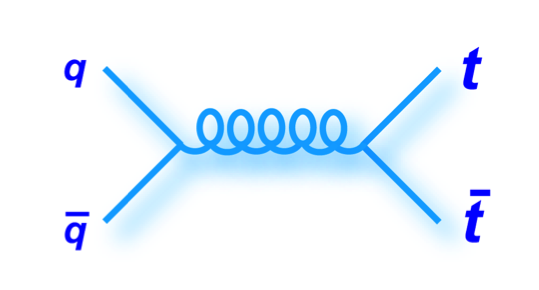
\includegraphics[height=0.25\textheight]{./plots/ttbar_1.png}
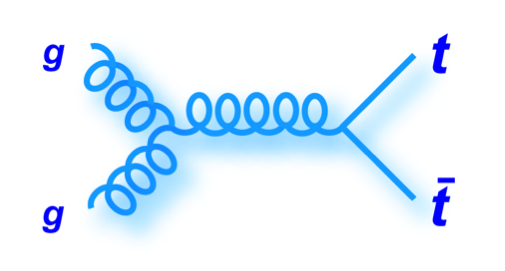
\includegraphics[height=0.25\textheight]{./plots/ttbar_2.png}
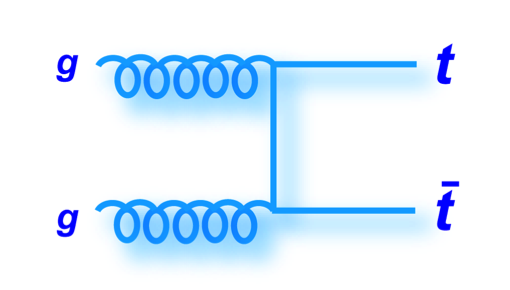
\includegraphics[height=0.25\textheight]{./plots/ttbar_3.png}
\begin{enumerate}
\item[o] The top quark is the heaviest elementary particle $\rightarrow$ largest Yukawa coupling.
\end{enumerate}
\centering
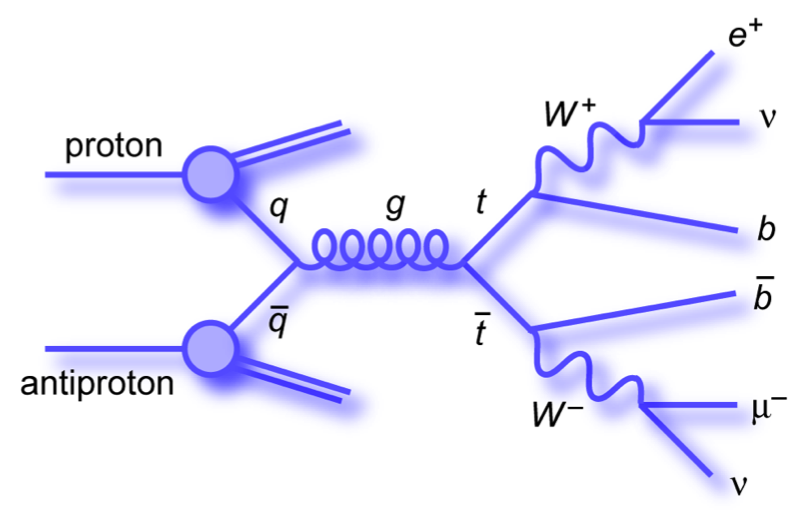
\includegraphics[height=0.3\textheight]{./plots/ttbar_4.png}
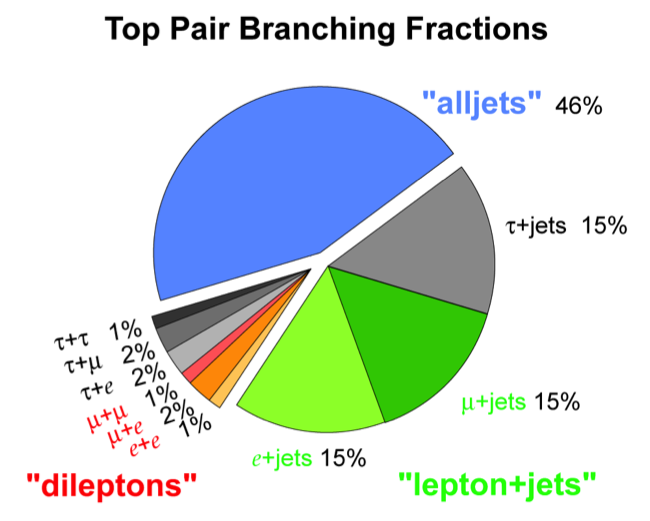
\includegraphics[height=0.3\textheight]{./plots/ttbar_5.png}
\begin{enumerate}
\item[o] Our analysis is top-quark pair-production in $e-\mu$ (2\% of ttbar).
\end{enumerate}
\end{frame}
\clearpage


\begin{frame} {Theoretical simulation vs. experimental analysis}
\begin{enumerate}
\item[o] Theoretical simulation: generated (truth) are known $\rightarrow$ observed (reco).
\item[o] Experimental analysis: observed (reco) are known $\rightarrow$ truth (nature)
\end{enumerate}
\centering
\includegraphics[height=0.53\textheight]{../output_20GeV/NN_plot1D_train_jetPt_truth_reco.pdf}
\includegraphics[height=0.53\textheight]{../output_20GeV/NN_plot1D_test_jetPt_truth_reco.pdf}
\begin{enumerate}
\item[o] The shapes of the distributions of the truth and reco observables for the training of the unfolding are very similar, but not identical (especially in the first bins). 
\end{enumerate}
\end{frame}
\clearpage


\begin{frame} {The 2D histogram of the migration matrix}
\begin{enumerate}
\item[o] The migration matrix between truth and reco is used in the traditional unfolding.
\item[o] Unfolding = inferring the generated (truth) from the observed (reconstructed).
\end{enumerate}
\centering
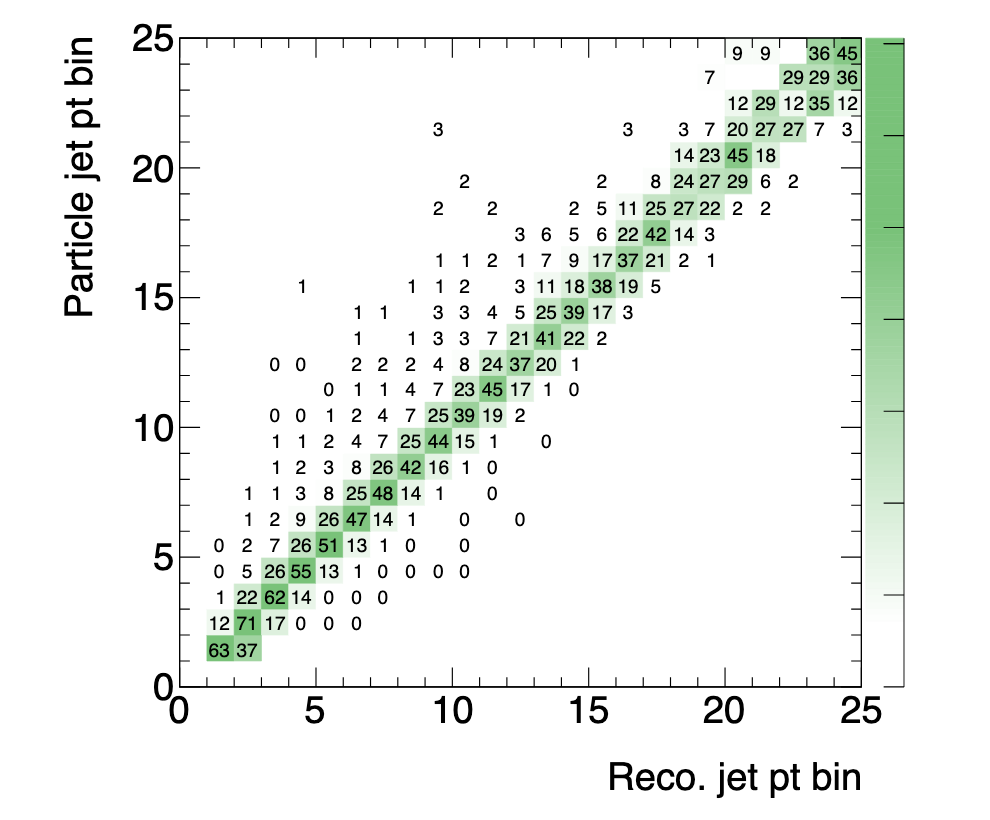
\includegraphics[height=0.42\textheight]{./plots/jetPt_migration_matrix.png}
\begin{enumerate}
\item[o] Plot from the same data, from the \href{http://www.desy.de/~liyichen/Unfolding.pdf}{report of Yichen Li}. The number in a cell represents the probability of an event in the truth bin i to be reconstructed in a reco bin j.
\item[o] The more diagonalizable matrix, the easier unfolding will be.
\item[o] Events are migrating from one truth bin to other bins for reco, and vice-versa.
\end{enumerate}
\end{frame}
\clearpage


\begin{frame}{A new approach: use machine learning to \emph{learn} how to unfold observed (reco) to true (generated).}
\begin{enumerate}
\item[o] \href{https://arxiv.org/pdf/1712.01814.pdf}{arXiv:1712:01814}
\end{enumerate}
\centering
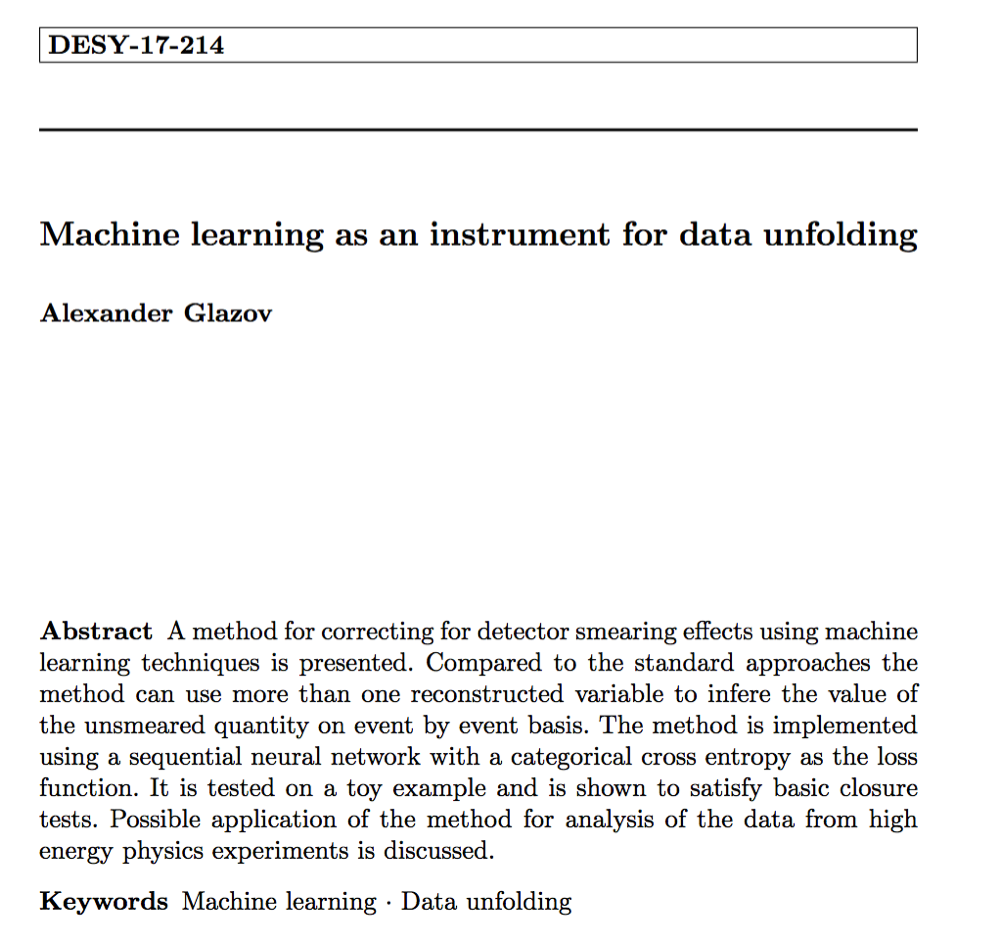
\includegraphics[height=0.7\textheight]{./plots/PaperToyData.png}
\end{frame}
\clearpage

\begin{frame}{Two unfolding methods: traditional and ML.}
\begin{enumerate}
\item[o] Traditional: binned migration matrix with only one variable.
\item[o] Machine learning: a continuous function of several variables.
\end{enumerate}
\centering
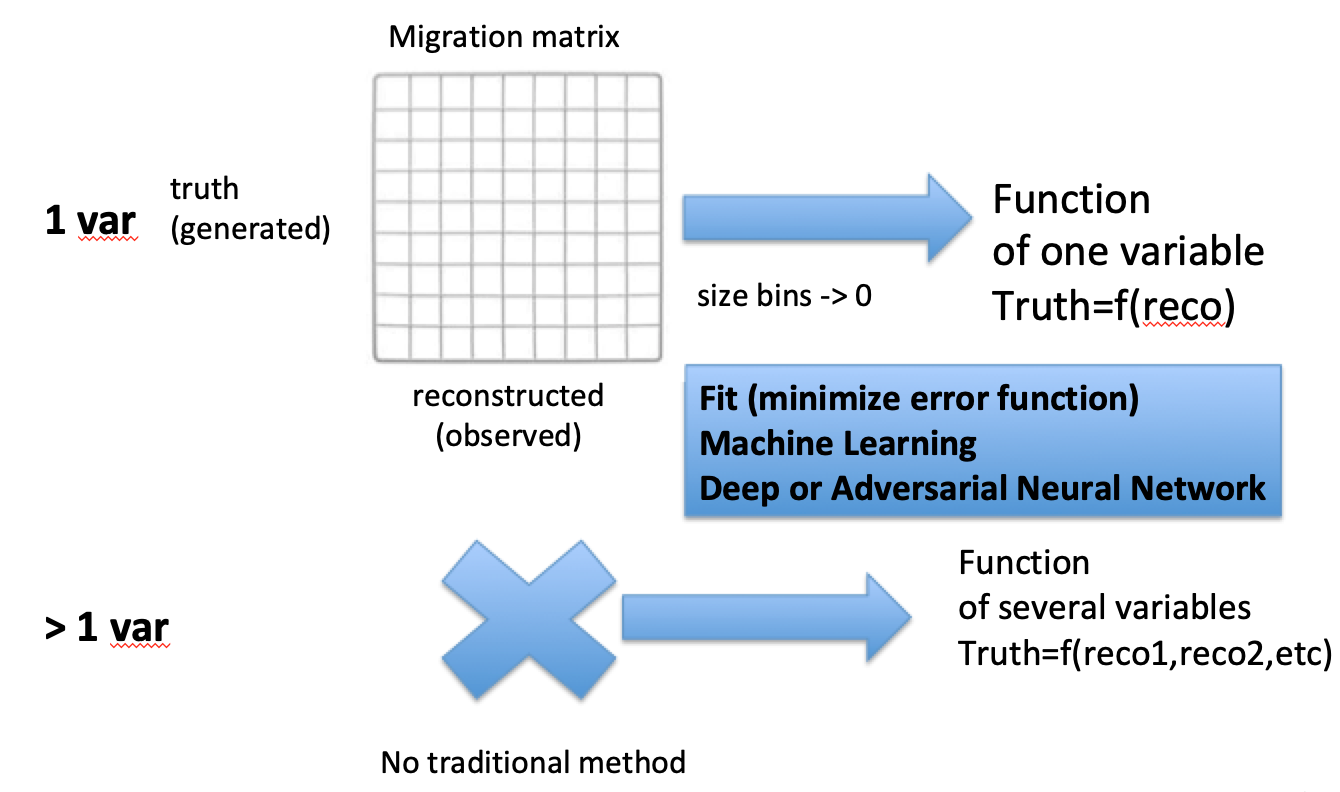
\includegraphics[height=0.70\textheight]{./plots/Unfolding_Traditional_ML.png}
\end{frame}
\clearpage

\begin{frame}{Physics problem: index of truth jet pt = f (reco jet pt) = ?}
\centering
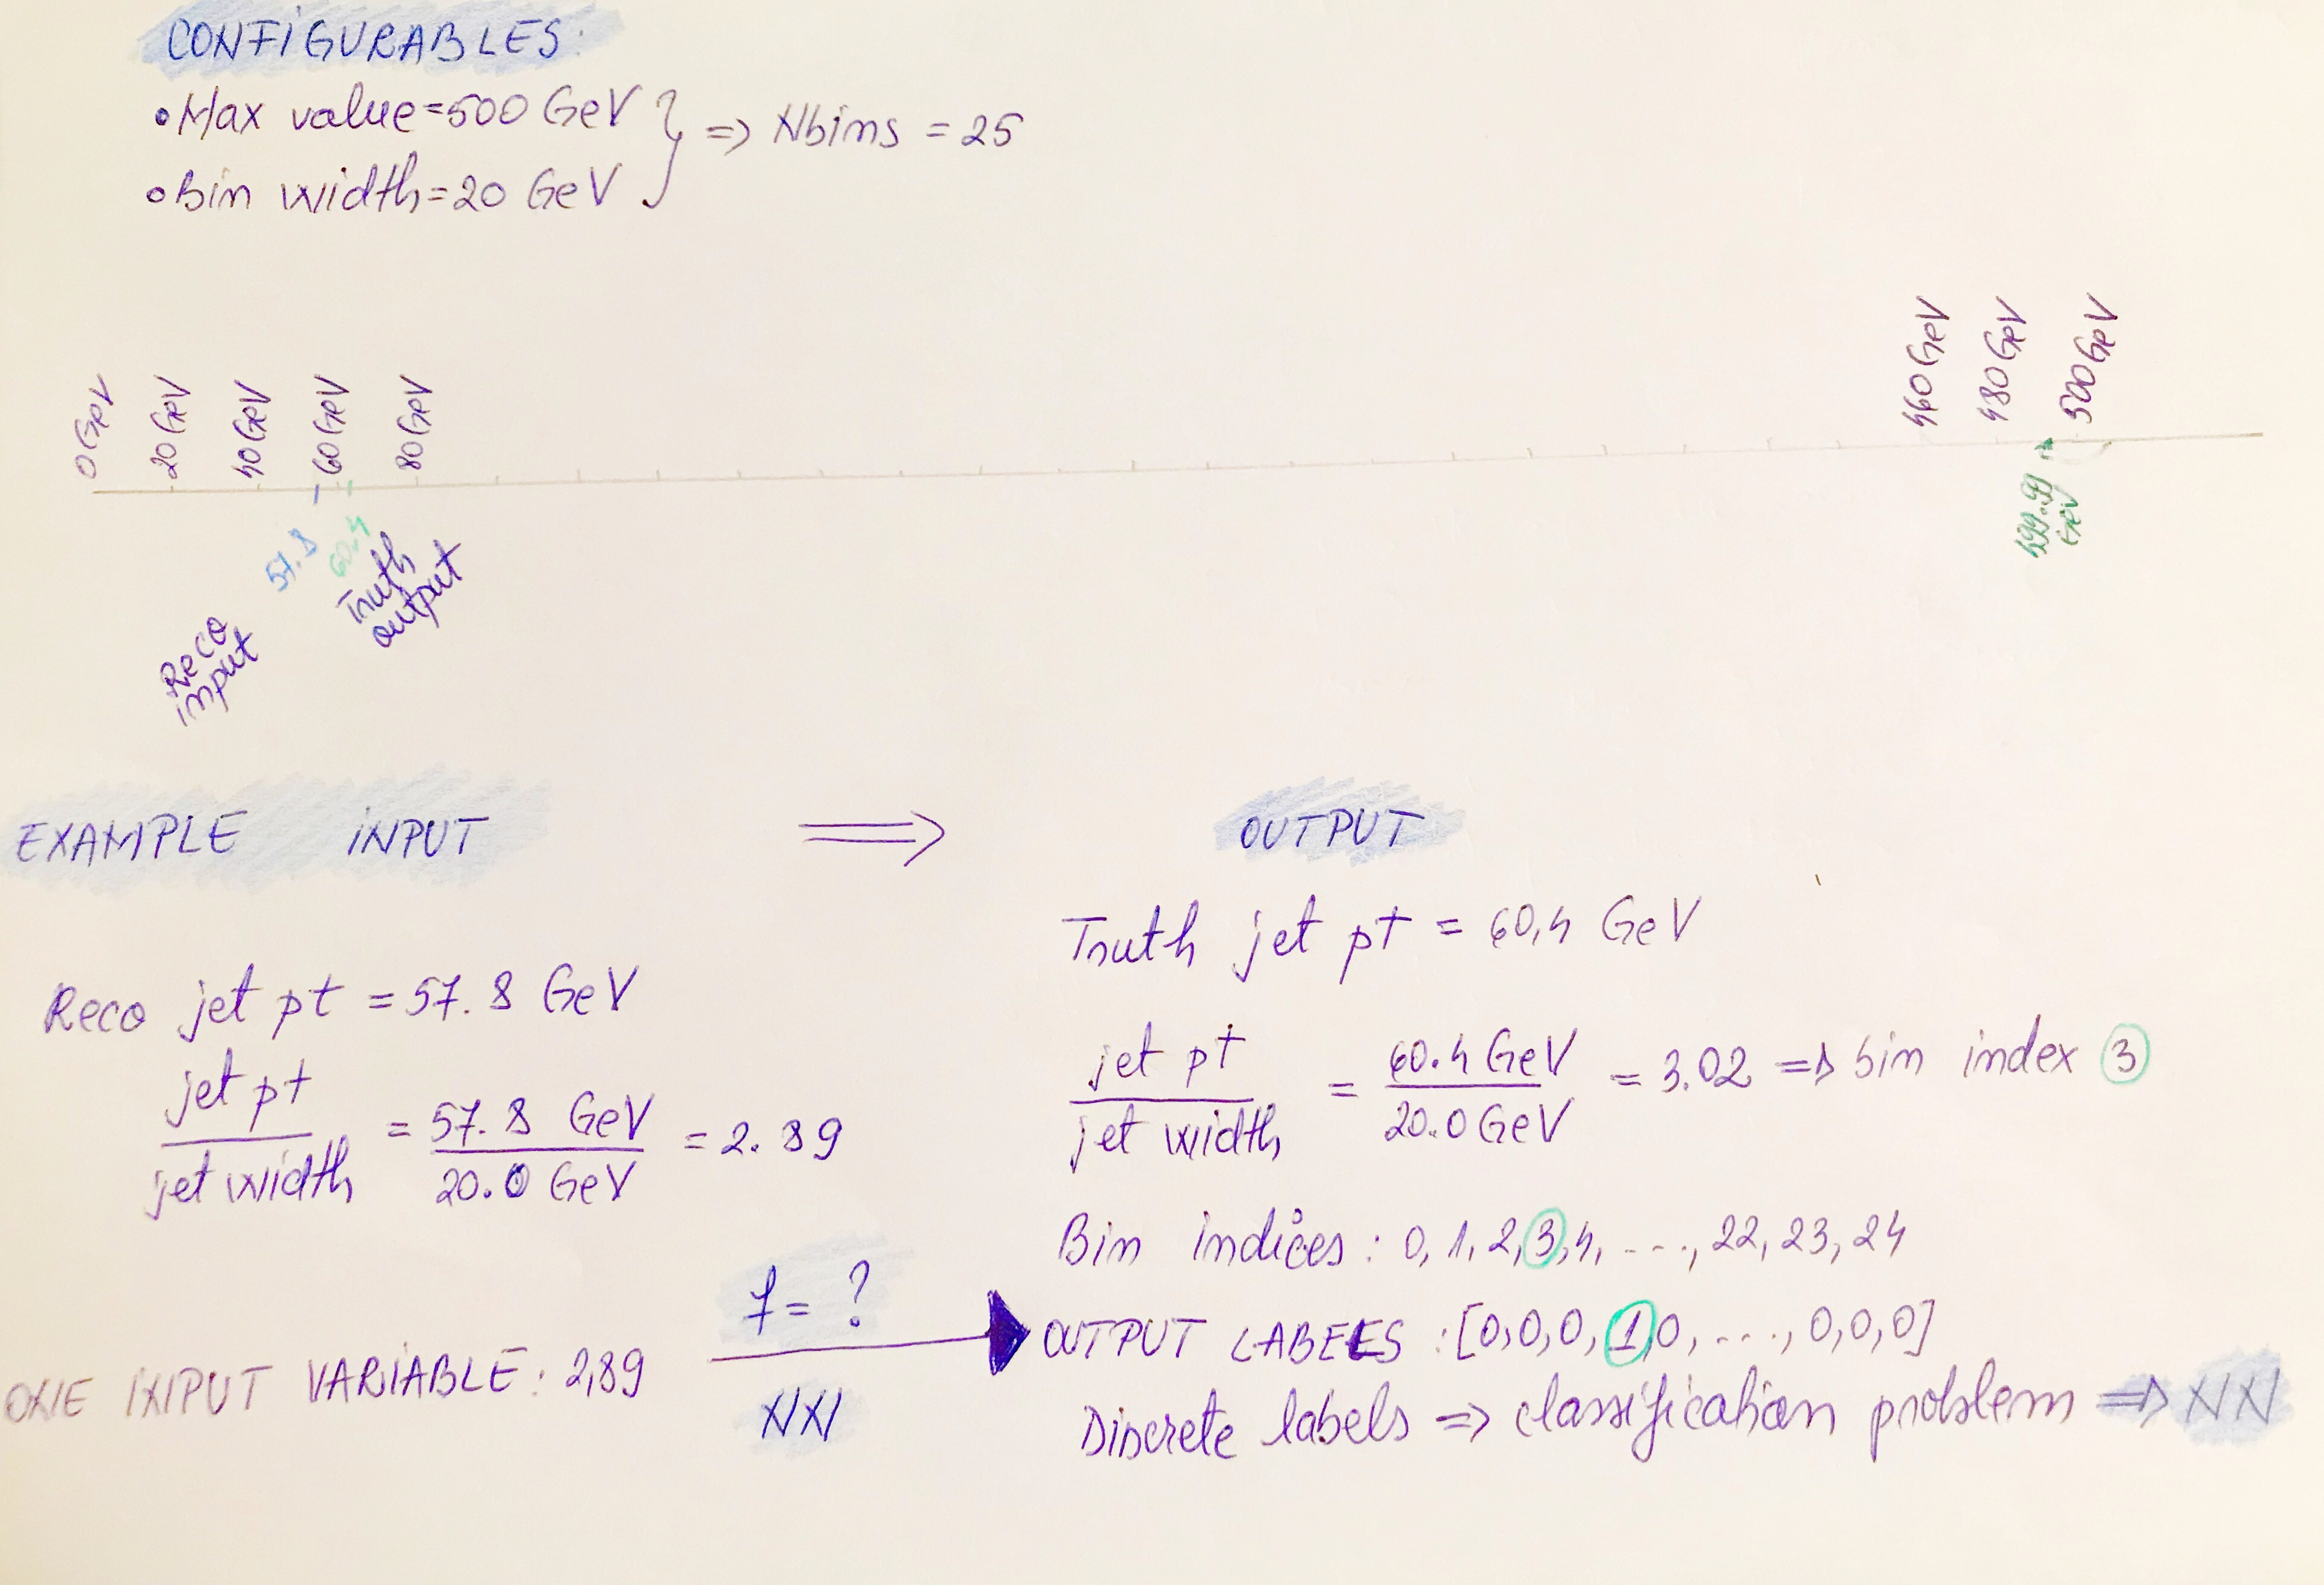
\includegraphics[height=0.80\textheight]{./plots/PhysicsProblem.jpg}
\end{frame}
\clearpage

\begin{frame}{The solution is using these NN architectures.}
\centering
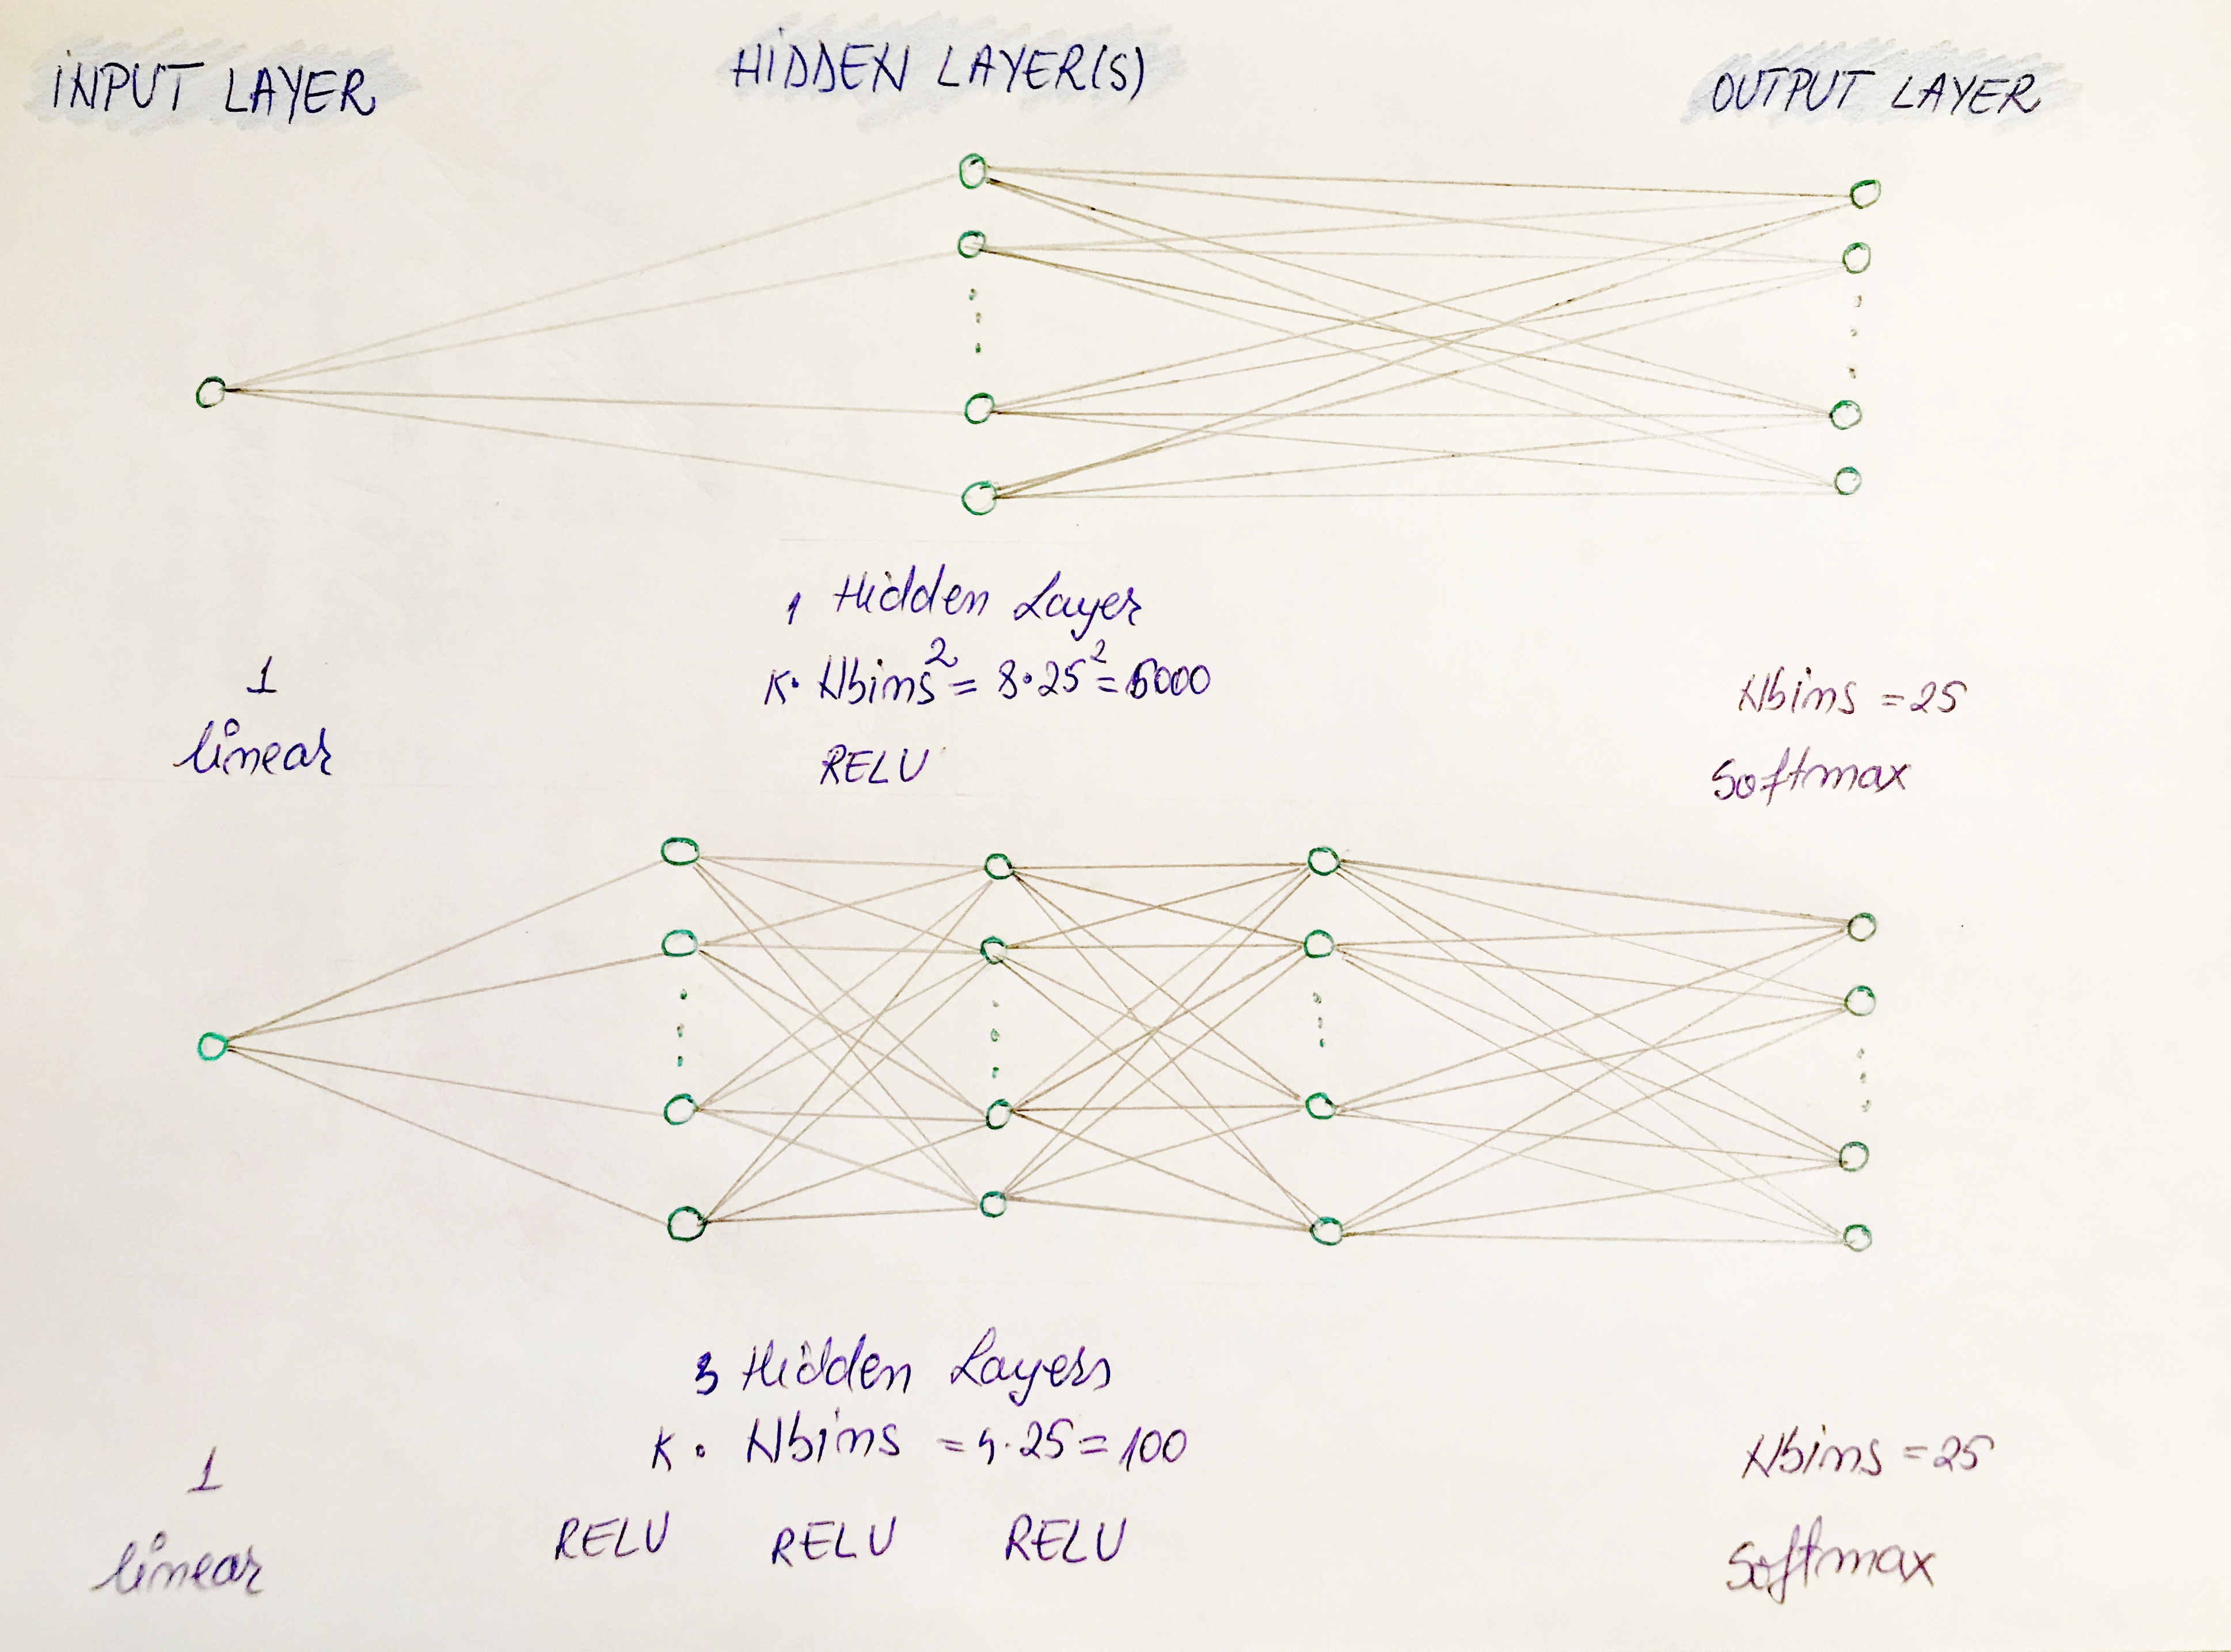
\includegraphics[height=0.80\textheight]{./plots/NNArchitecture.jpg}
\end{frame}
\clearpage

\begin{frame}{The NN is implemented in TensorFlow, via Keras, in Python.}
\centering

\includegraphics[height=0.25\textheight]{./plots/TensorFlow_Keras.png}

\includegraphics[height=0.25\textheight]{./plots/Python.png}
\begin{enumerate}
\item[o] Ran the DNN software for unfolding by DESY Hamburg.
\item[o] Ran on lxplus using the ML software docker image via singularity.
\item[o] Read the ROOT file via the uproot package.
\item[o] Trained  the NNs in Python using Keras and TensorFlow.
\end{enumerate}
\ \\
\ \\
\begin{enumerate}
\item[o] Fine tuned the NN hyper parameters for our ROOT data sample.
\item[o] One NN training is the first step of the iterative unfolding procedure. 
\end{enumerate}
\end{frame}
\clearpage

\begin{frame}{Summary of the physics and NN choices}
\begin{table}[h!]
\begin{enumerate}
\item[o] One file with 43076 events (and leading jets). Half (21538) in training, half in testing. 
\item[o] jet pt: range=0-500 GeV, bin width=20 GeV, number of bins = 500/20 = 25.
\item[o] Chose the NN training hyper-parameters by changing one at a time while keeping the other constant, and choosing those with largest accuracy and smallest loss values.
\end{enumerate}
  \resizebox{\textwidth}{!}{
    \begin{tabular}{|l|l|l|} % <-- Alignments: 1st column left, 2nd middle and 3rd right, with vertical lines in between
      \hline
      \textbf{Choice} & \textbf{Old NN (toy data example)} & \textbf{New NN (my best choice)}\\
      \hline
      number of nodes per input layer & 1 & 1 \\
      number of nodes per output layer & ${\rm Nbins}=25$ & ${\rm Nbins}=25$ \\
      Number of hidden layers & 1 & 3 \\
      ${\rm k}$ & 8 & 4 \\
      Number of nodes per layer & ${\rm k}\cdot {\rm Nbins}^2=5000$ & ${\rm k}\cdot {\rm Nbins}=100$ \\
      activation function input & linear & linear \\
      activation function hidden & ReLU & ReLU \\
      activation function output & softmax & softmax \\
      batch size & 1000 & 200 \\
      number of epochs & 150 & 150 \\
      \hline
    \end{tabular}
  }
\end{table}
\end{frame}
\clearpage

\begin{frame}{Two figures of merit to optimise the NN hyper-parameters}
\begin{enumerate}
\item[o] The accuracy: the larger, the better (left: old NN; right: new NN).
\end{enumerate}
\centering
\includegraphics[height=0.28\textheight]{../output_20GeV/NN_plot1D_optionTrainTest_accuracy_NN_l_A1_k_8_e_150_b_1000.pdf}
\includegraphics[height=0.28\textheight]{../output_20GeV/NN_plot1D_optionTrainTest_accuracy_NN_l_B3_k_4_e_150_b_200.pdf}\\
\begin{enumerate}
\item[o] The loss (error) value: the smaller, the better (left: old NN; right: new NN).
\end{enumerate}
\centering
\includegraphics[height=0.28\textheight]{../output_20GeV/NN_plot1D_optionTrainTest_loss_NN_l_A1_k_8_e_150_b_1000.pdf}
\includegraphics[height=0.28\textheight]{../output_20GeV/NN_plot1D_optionTrainTest_loss_NN_l_B3_k_4_e_150_b_200.pdf}\\
\begin{enumerate}
\item[o] Overlaid \textcolor{cyan}{train} and \textcolor{magenta}{test} are very similar $\rightarrow$ we did not overtrain the NNs. 
\end{enumerate}
\end{frame}
\clearpage

\begin{frame}{Overlaying the two NN architectures: \textcolor{red}{old} and \textcolor{OliveGreen}{new}. }
\begin{enumerate}
\item[o] The accuracy: the larger, the better (left: train; right: test).
\end{enumerate}
\centering
\includegraphics[height=0.28\textheight]{../output_20GeV/NN_plot1D_train_accuracy_NN_final.pdf}
\includegraphics[height=0.28\textheight]{../output_20GeV/NN_plot1D_test_accuracy_NN_final.pdf}\\
\begin{enumerate}
\item[o] The loss (error) value: the smaller, the better (left: train; right: test).
\end{enumerate}
\centering
\includegraphics[height=0.28\textheight]{../output_20GeV/NN_plot1D_train_loss_NN_final.pdf}
\includegraphics[height=0.28\textheight]{../output_20GeV/NN_plot1D_test_loss_NN_final.pdf}\\
\begin{enumerate}
\item[o] The \textcolor{OliveGreen}{new} NN architecture outperforms the \textcolor{red}{old} one.
\end{enumerate}
\end{frame}
\clearpage

\begin{frame}{The jet pt distribution as the index of the jet pt bin.}
\begin{enumerate}
\item[o] True output (generated, truth) vs input (reconstructed). Used in traditional unfolding.
\end{enumerate}
\centering
\includegraphics[height=0.27\textheight]{../output_20GeV/NN_plot1D_train_jetPtBin_NN_noTrained.pdf}
\includegraphics[height=0.27\textheight]{../output_20GeV/NN_plot1D_test_jetPtBin_NN_noTrained.pdf}
\begin{enumerate}
\item[o] The true output vs the predicted unfolded output by each NN architecture.
\item[o] The \textcolor{OliveGreen}{new} NN architecture is closer to the \textcolor{blue}{true output} than the \textcolor{red}{old} one.
\end{enumerate}
\centering
\includegraphics[height=0.27\textheight]{../output_20GeV/NN_plot1D_train_jetPtBin_NN_final.pdf}
\includegraphics[height=0.27\textheight]{../output_20GeV/NN_plot1D_test_jetPtBin_NN_final.pdf}
\end{frame}
\clearpage

\begin{frame}{The predicted NN output minus the true output.}
\begin{enumerate}
\item[o] Both outputs are integers, representing bin indices, $\rightarrow$ difference = also integer.
\item[o] The greater the count at zero difference, the better.
\item[o] Top: train, bottom: test. Left to right, bin widths of 10, 20, 50, 100 GeV.
\item[o] The smaller the binWidth, the better is the \textcolor{OliveGreen}{new} NN architecture relative to the \textcolor{red}{old} one.
\end{enumerate}
\centering
\includegraphics[height=0.25\textheight]{../output_10GeV/NN_plot1D_train_outputPredictedMinusTrue_NN_final.pdf}
\includegraphics[height=0.25\textheight]{../output_20GeV/NN_plot1D_train_outputPredictedMinusTrue_NN_final.pdf}
\includegraphics[height=0.25\textheight]{../output_50GeV/NN_plot1D_train_outputPredictedMinusTrue_NN_final.pdf}
\includegraphics[height=0.25\textheight]{../output_100GeV/NN_plot1D_train_outputPredictedMinusTrue_NN_final.pdf}\\
\includegraphics[height=0.25\textheight]{../output_10GeV/NN_plot1D_test_outputPredictedMinusTrue_NN_final.pdf}
\includegraphics[height=0.25\textheight]{../output_20GeV/NN_plot1D_test_outputPredictedMinusTrue_NN_final.pdf}
\includegraphics[height=0.25\textheight]{../output_50GeV/NN_plot1D_test_outputPredictedMinusTrue_NN_final.pdf}
\includegraphics[height=0.25\textheight]{../output_100GeV/NN_plot1D_test_outputPredictedMinusTrue_NN_final.pdf}
\end{frame}
\clearpage

\begin{frame}{The 2D histogram migration matrix of the index of the jet pt}
\begin{enumerate}
\item[o] The closer to a diagonal matrix, the better.
\item[o] Top: train, Bottom: test.
\item[o] Left to right: input, \textcolor{red}{old} NN output, \textcolor{OliveGreen}{new} NN output vs true output. 
\end{enumerate}
\centering
\includegraphics[height=0.25\textheight]{../output_20GeV/NN_plot2D_train_outputTrue_input.pdf}
\includegraphics[height=0.25\textheight]{../output_20GeV/NN_plot2D_train_outputTrue_outputPredicted_NN_l_A1_k_8_e_150_b_1000.pdf}
\includegraphics[height=0.25\textheight]{../output_20GeV/NN_plot2D_train_outputTrue_outputPredicted_NN_l_B3_k_4_e_150_b_200.pdf}\\
\includegraphics[height=0.25\textheight]{../output_20GeV/NN_plot2D_test_outputTrue_input.pdf}
\includegraphics[height=0.25\textheight]{../output_20GeV/NN_plot2D_test_outputTrue_outputPredicted_NN_l_A1_k_8_e_150_b_1000.pdf}
\includegraphics[height=0.25\textheight]{../output_20GeV/NN_plot2D_test_outputTrue_outputPredicted_NN_l_B3_k_4_e_150_b_200.pdf}\\
\end{frame}
\clearpage

\begin{frame}{Traditional unfolding results}
\begin{enumerate}
\item[o] Plot taken from Fig. 5 of \href{http://www.desy.de/~liyichen/Unfolding.pdf}{study by Yichen Li}.
\item[o] Traditional unfolding: iterative bayesian unfolding with 4 iterations.
\end{enumerate}
\centering
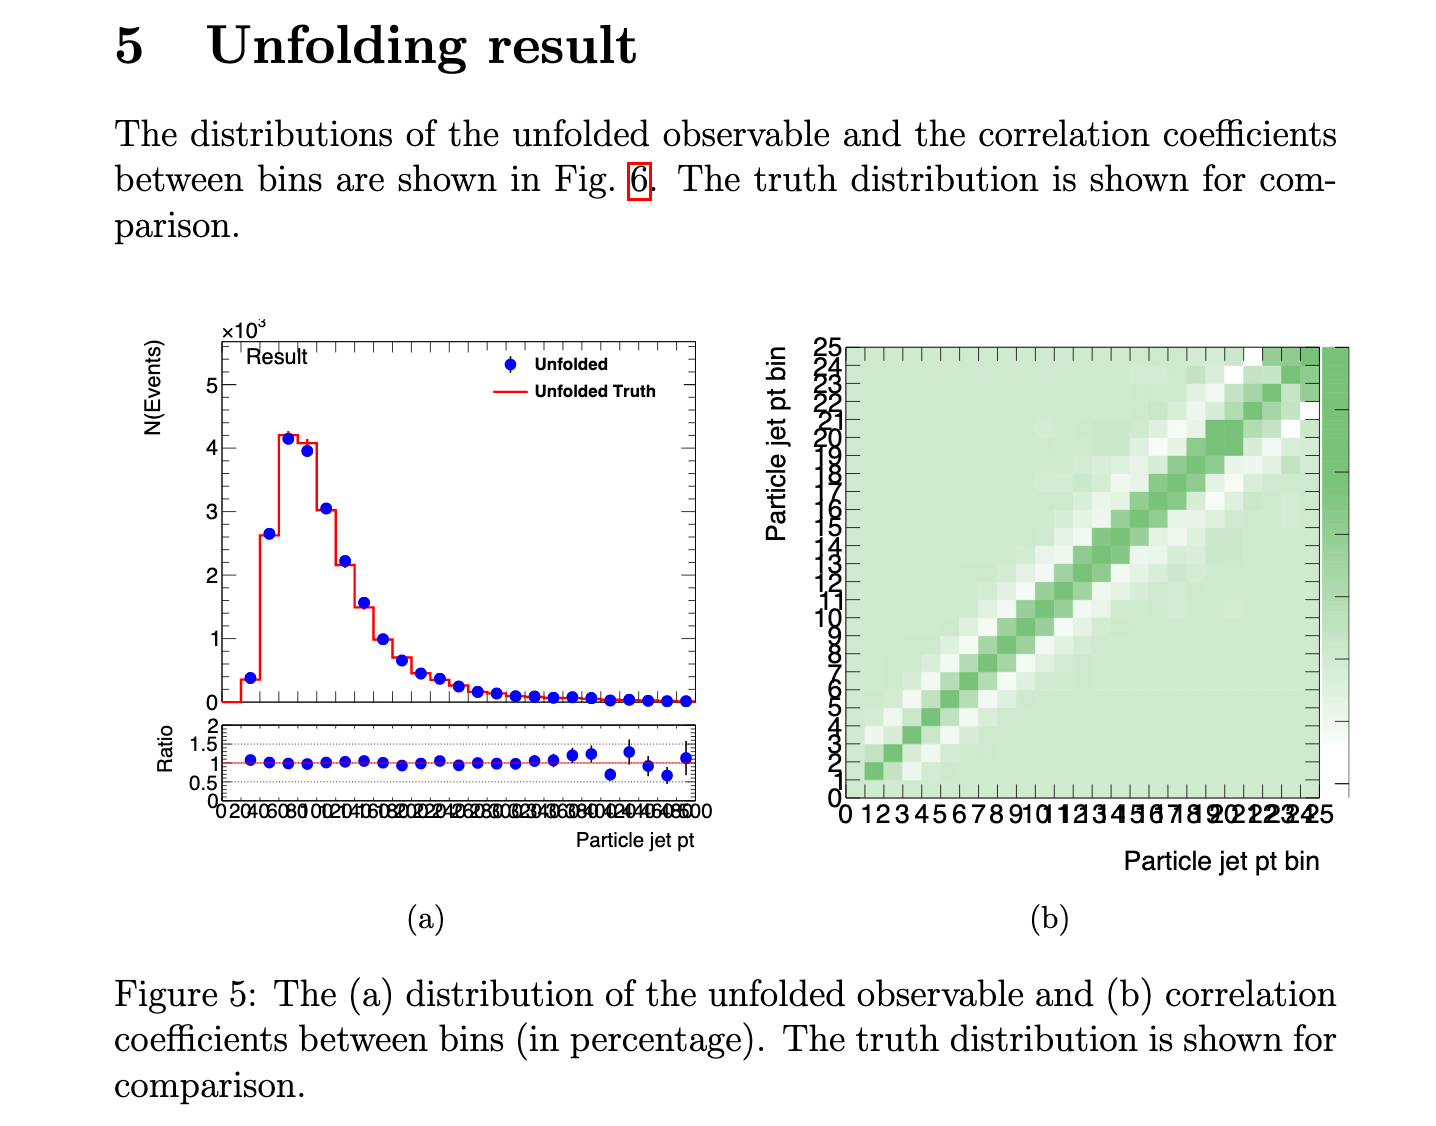
\includegraphics[height=0.65\textheight]{./plots/TraditionalUnfolding.png}
\end{frame}
\clearpage

\begin{frame}{Summary and Next Steps}
\begin{enumerate}
\item[o] Studied Unfolding of the jet pt distributions in ttbar e-mu analysis.
\item[o] Bin of truth jet pt = f (reco jet pt) = ?
\item[o] Discrete output values  $\rightarrow$ classification problem $\rightarrow$ NN.
\item[o] Coded using Tensor Flow via Keras in Python.
\item[o] Followed code example with toy data in arXiv (\href{https://arxiv.org/pdf/1712.01814.pdf}{link for arXiv:1712:01814}).
\item[o] Fine tuned NN hyper-parameters and architecture for our jet data.
\item[o] The chosen NN outperforms the one from the toy data.
\item[o] The project code and report are in GitLab (\href{https://gitlab.cern.ch/lciucu/MLUnfolding/}{link}).
\end{enumerate}
\ \\
\ \\
\begin{enumerate}
\item[o] Training recursively several NNs of the found architecture.
\begin{enumerate}
\item[o] One NN training is just the first (zeroth) step in the NN unfolding method.
\end{enumerate}
\item[o] Use more data (more events and leading jets).
\item[o] Add other input variables (e.g. jet $\eta$).
\item[o] Instead of k-fold=2 (train and test at 50\%), use a larger k-fold (e.g. 5).
\end{enumerate}
\end{frame}
\clearpage

\begin{frame}{Backup slides}
\end{frame}
\clearpage

